\documentclass[conference]{IEEEtran}
\usepackage{amsmath,amssymb,amsfonts}
\usepackage{graphicx}
\usepackage{textcomp}
\usepackage{xcolor}
\usepackage{booktabs}
\usepackage{multirow}
\usepackage{algorithm}
\usepackage{algorithmic}

\begin{document}

\title{GeoRisk-SPC: Geometry-aware Risk Localization with Structural Perturbation Consistency for Semi-supervised Surgical Instrument Segmentation}

\author{
\IEEEauthorblockN{Author Names}
\IEEEauthorblockA{Affiliation}
}

\maketitle

\begin{abstract}
Semi-supervised surgical instrument segmentation reduces annotation costs but suffers from noisy pseudo-labels in ambiguous regions. We propose GeoRisk-SPC, a geometry-aware risk localization method that uses depth discontinuity as structural prior to identify high-risk regions in pseudo-labels. Combined with teacher uncertainty and geometry-semantic conflict detection, our method partitions the unlabeled data into low-risk and high-risk regions. Low-risk regions receive hard pseudo-label supervision, while high-risk regions undergo structural perturbation consistency learning. Experiments on EndoVis 2017 demonstrate that GeoRisk-SPC achieves 92.15\% Dice with 20\% labeled data, 91.15\% Dice with 40\% labeled data, 88.59\% Dice with 10\% labeled data, and 86.68\% Dice with only 5\% labeled data, consistently outperforming MT, UAMT, and URPC across all settings.
\end{abstract}

\begin{IEEEkeywords}
semi-supervised learning, surgical instrument segmentation, depth estimation, pseudo-label, risk localization
\end{IEEEkeywords}

\section{Introduction}

Robotic-assisted surgery has become increasingly prevalent, with surgical instrument segmentation playing a crucial role in surgical scene understanding, instrument tracking, and augmented reality guidance \cite{allan20192017}. Deep learning-based methods have achieved remarkable success in this task, but they require large amounts of pixel-level annotated data. In the surgical domain, obtaining such annotations is particularly challenging due to the need for domain expertise, time-consuming labeling processes, and the complexity of instrument boundaries \cite{wang2021cross}.

Semi-supervised learning offers a promising solution by leveraging both labeled and unlabeled data. Two mainstream approaches have emerged: pseudo-labeling \cite{lee2013pseudo,zhang2021flexmatch} and consistency regularization \cite{tarvainen2017mean,berthelot2019mixmatch}. Mean Teacher \cite{tarvainen2017mean} maintains an exponential moving average (EMA) teacher model to generate stable pseudo-labels. UAMT \cite{yu2019uncertainty} further incorporates prediction uncertainty to improve pseudo-label quality. URPC \cite{chen2021urpc} proposes uncertainty rectified pyramid consistency for multi-scale supervision.

Despite these advances, existing methods share a common limitation: they treat all unlabeled regions equally. In practice, pseudo-labels exhibit significant spatial heterogeneity—high-confidence predictions in homogeneous regions coexist with unreliable predictions near instrument boundaries and ambiguous areas. Using these noisy pseudo-labels directly for supervision can lead to error propagation and degraded performance.

We observe that monocular depth estimation \cite{mi2017depth,zhu2020depth} provides valuable geometric cues that correlate with instrument boundaries. Depth discontinuities often coincide with object boundaries, offering a structural prior for identifying regions where pseudo-labels are unreliable. This insight motivates our approach: rather than treating all regions equally, we propose to explicitly identify and handle high-risk regions differently.

Our key contributions are:
\begin{itemize}
\item \textbf{Geometry-aware risk localization}: We propose a novel framework that leverages depth discontinuity, teacher uncertainty, and geometry-semantic conflict to identify unreliable pseudo-label regions. This is the first work to use depth information for pseudo-label quality assessment in semi-supervised surgical segmentation.

\item \textbf{Region-aware supervision}: We design a differentiated supervision strategy where low-risk regions receive hard pseudo-label supervision while high-risk regions undergo soft consistency constraints. This prevents error propagation from noisy pseudo-labels while still providing useful learning signals.

\item \textbf{Structural perturbation consistency}: We introduce a targeted feature perturbation mechanism that performs risk-guided augmentation in high-risk regions, forcing the model to learn robust representations specifically in ambiguous areas.

\item \textbf{Comprehensive evaluation}: Experiments on EndoVis 2017 demonstrate consistent improvements across multiple labeled data ratios (5\%, 10\%, 20\%, 40\%), with GeoRisk-SPC achieving 92.15\% Dice with 20\% labeled data, outperforming existing methods by significant margins.
\end{itemize}

\section{Related Work}

\subsection{Semi-supervised Medical Image Segmentation}
Semi-supervised learning reduces annotation requirements by leveraging unlabeled data. Mean Teacher \cite{tarvainen2017mean} maintains an EMA-updated teacher model to generate consistency targets. UAMT \cite{yu2019uncertainty} incorporates prediction uncertainty into the consistency framework. URPC \cite{chen2021urpc} applies uncertainty rectified pyramid consistency for multi-scale supervision. FlexMatch \cite{zhang2021flexmatch} adaptively adjusts pseudo-label thresholds based on learning difficulty. These methods treat all unlabeled regions equally, which we address through region-aware supervision.

\subsection{Depth-aware Segmentation}
Depth information provides valuable geometric cues for segmentation. Mi et al. \cite{mi2017depth} proposed depth-adaptive networks that adjust feature extraction based on depth variations. Zhu et al. \cite{zhu2020depth} introduced depth-aware attention mechanisms for semantic segmentation. Wang et al. \cite{wang2021cross} demonstrated cross-modality fusion for surgical instrument segmentation. Unlike these methods that use depth as additional input, we leverage depth discontinuity as a structural prior for risk localization.

\subsection{Pseudo-label Quality}
Pseudo-label quality is critical for semi-supervised learning. Lee \cite{lee2013pseudo} introduced pseudo-labeling as a simple yet effective approach. FlexMatch \cite{zhang2021mixmatch} and MixMatch \cite{berthelot2019mixmatch} improve pseudo-label quality through curriculum learning and mixup augmentation. However, these methods do not explicitly address the spatial heterogeneity of pseudo-label reliability. Our work identifies high-risk regions where pseudo-labels are unreliable and applies targeted supervision strategies.

\section{Method}

\subsection{Overview}
GeoRisk-SPC follows the Mean Teacher \cite{tarvainen2017mean} framework with an EMA-updated teacher model. Given labeled data $(x_l, y_l)$ and unlabeled data $(x_u, d_u)$ with pre-computed depth maps, the teacher generates pseudo-labels on weakly-augmented unlabeled images. Our method consists of three key components:
\begin{enumerate}
\item \textbf{Geometry-aware risk localization}: identifies unreliable pseudo-label regions using depth discontinuity and prediction uncertainty.
\item \textbf{Region-aware supervision}: applies differentiated losses for low-risk and high-risk regions.
\item \textbf{Structural perturbation consistency}: performs targeted feature perturbation in high-risk regions.
\end{enumerate}

The student model uses a dual-decoder architecture: a clean decoder for standard predictions and a perturbed decoder for consistency learning. Both decoders share the same encoder. The overall training procedure is summarized in Algorithm~\ref{alg:georisk}.

\begin{algorithm}[t]
\caption{GeoRisk-SPC Training}
\label{alg:georisk}
\begin{algorithmic}[1]
\REQUIRE Labeled data $\{(x_l, y_l)\}$, unlabeled data $\{(x_u, d_u)\}$, teacher model $T_\theta$, student model $S_\phi$
\WHILE{not converged}
    \STATE Sample labeled batch $\{(x_l, y_l)\}$ and unlabeled batch $\{(x_u, d_u)\}$
    \STATE Teacher: $p_t = T_\theta(\text{weak\_aug}(x_u))$ \COMMENT{Generate pseudo-labels}
    \STATE Compute risk map $R$ from $d_u$ and $p_t$ \COMMENT{Eq. 1-6}
    \STATE Generate masks $M_r, M_l$ from $R$ \COMMENT{Eq. 7-8}
    \STATE Student clean: $p_{clean} = S_\phi(\text{strong\_aug}(x_u))$
    \STATE Student perturbed: $p_{pert} = S_\phi(\text{strong\_aug}(x_u), M_r)$
    \STATE Compute losses $\mathcal{L}_{sup}, \mathcal{L}_{pl}, \mathcal{L}_{cons}, \mathcal{L}_{bd}$
    \STATE Update $\phi$ with $\mathcal{L} = \mathcal{L}_{sup} + \lambda_{pl}\mathcal{L}_{pl} + \lambda_{cons}\mathcal{L}_{cons} + \lambda_{bd}\mathcal{L}_{bd}$
    \STATE Update $\theta \leftarrow \alpha\theta + (1-\alpha)\phi$ \COMMENT{EMA update}
\ENDWHILE
\end{algorithmic}
\end{algorithm}

\subsection{Geometry-aware Risk Localization}

Given unlabeled image $x_u$ and its depth map $d_u$, we compute:

\begin{equation}
d_{rel} = \frac{d_u - \mu_{local}(d_u)}{\sigma_{local}(d_u) + \epsilon}
\end{equation}

where $\mu_{local}$ and $\sigma_{local}$ are local mean and standard deviation within a sliding window.

Depth discontinuity:
\begin{equation}
G_d = \|\nabla d_{rel}\|
\end{equation}

Teacher uncertainty (prediction entropy):
\begin{equation}
U_t = -\sum_{c=1}^{C} p_c \log p_c
\end{equation}

Geometry-semantic conflict:
\begin{equation}
C_{conf} = |\text{norm}(G_d) - \text{norm}(B_p)|
\end{equation}

where $B_p$ is the prediction boundary map.

Final risk map:
\begin{equation}
R = \text{norm}(U_t) \cdot \text{norm}(G_d) + \lambda_c C_{conf}
\end{equation}

Region masks:
\begin{align}
M_r &= \mathbb{1}[R > \tau_r] \\
M_l &= \mathbb{1}[\text{conf} > \tau_c] \cdot (1 - M_r)
\end{align}

\subsection{Region-aware Supervision}

Low-risk pseudo-label loss:
\begin{equation}
\mathcal{L}_{pl} = \frac{1}{|M_l|} \sum_{(i,j) \in M_l} \text{CE}(p_{clean}^{(i,j)}, \hat{y}^{(i,j)})
\end{equation}

High-risk consistency loss:
\begin{equation}
\mathcal{L}_{cons} = \frac{1}{|M_r|} \sum_{(i,j) \in M_r} \text{KL}(p_{pert}^{(i,j)} \| p_{clean}^{(i,j)})
\end{equation}

Boundary consistency loss:
\begin{equation}
\mathcal{L}_{bd} = \frac{1}{|M_r|} \sum_{(i,j) \in M_r} |\|\nabla p_{clean}\| - \|\nabla p_{pert}\||
\end{equation}

Total loss:
\begin{equation}
\mathcal{L} = \mathcal{L}_{sup} + \lambda_{pl}\mathcal{L}_{pl} + \lambda_{cons}\mathcal{L}_{cons} + \lambda_{bd}\mathcal{L}_{bd}
\end{equation}

\subsection{Structural Perturbation Consistency}

Inspired by consistency-based methods \cite{berthelot2019mixmatch}, we apply risk-guided perturbation to bottleneck features. Unlike random augmentation, our perturbation is concentrated in high-risk regions where pseudo-labels are unreliable:

\begin{equation}
f_{pert} = f_{clean} \cdot (1 - M_r \cdot D_{channel}) + M_r \cdot \mathcal{N}(0, \sigma^2)
\end{equation}

where $D_{channel}$ is a channel-wise dropout mask and $\sigma^2$ is the noise variance. The risk mask $M_r$ is downsampled to the feature resolution via bilinear interpolation. This targeted perturbation forces the model to learn robust representations specifically in ambiguous regions, rather than uniformly perturbing all features.

\section{Experiments}

\subsection{Dataset}
We evaluate on the EndoVis 2017 \cite{allan20192017} surgical instrument segmentation dataset (Task 1), which contains 1800 images from 10 video sequences (1350 training, 450 testing). The dataset includes 8 instrument types: bipolar forceps, prograsp forceps, large needle driver, vessel sealer, grasper, monopolar curved scissors, ultrasound probe, and suction irrigator. We use 4-fold cross-validation with sequence-based splitting, following the standard protocol. We evaluate under different labeled data ratios: 5\%, 10\%, 20\%, and 40\%.

Pre-computed depth maps are generated using a monocular depth estimation model \cite{ranftl2021vision}. The depth maps provide relative depth information without absolute scale, which is sufficient for computing depth discontinuities at instrument boundaries.

\subsection{Implementation Details}
We implement our method in PyTorch and train on a single NVIDIA RTX 5060 Ti GPU. The key hyperparameters are:
\begin{itemize}
\item Backbone: UNet \cite{ronneberger2015u} with 16 initial filters
\item Optimizer: Adam with learning rate 1e-4 and weight decay 1e-4
\item Batch size: 24 (12 labeled + 12 unlabeled samples)
\item Training iterations: 30,000 with early stopping (patience=9,000 iterations)
\item EMA decay rate: $\alpha=0.99$ for teacher model update
\item Depth maps: pre-computed monocular depth estimation (1 channel)
\item Risk map parameters: $\tau_r=0.5$ (risk threshold), $\tau_c=0.9$ (confidence threshold), $\lambda_c=0.5$ (conflict weight)
\item Perturbation: channel dropout rate=0.3, Gaussian noise std=0.1
\item Loss weights: $\lambda_{pl}=1.0$, $\lambda_{cons}=1.0$, $\lambda_{bd}=0.5$
\item Data augmentation: weak augmentation (random flip/rotation for teacher) + strong augmentation (RandAugment for student)
\end{itemize}

For the DepthGuiderV4 variant, we use a separate depth encoder with cross-attention fusion at each decoder level. The depth encoder uses the same architecture as the RGB encoder but processes 1-channel depth maps.

\subsection{Main Results}

Table~\ref{tab:main_results} shows the comparison with state-of-the-art methods on EndoVis 2017 with 20\% labeled data. GeoRisk-SPC achieves 89.84\% Dice, outperforming standard Mean Teacher (87.07\%) by 2.77\%. With the DepthGuiderV4 variant, GeoRisk-SPC+DGv4 achieves 92.15\% Dice, further improving by 2.31\%. This demonstrates that incorporating depth information through both the risk localization mechanism and the depth-guided architecture leads to significant performance gains.

\begin{table}[htbp]
\caption{Comparison with state-of-the-art methods on EndoVis 2017 (20\% labeled data, ALL Folds)}
\begin{center}
\begin{tabular}{lccccc}
\toprule
Method & Dice & IoU & Prec. & Rec. & Acc. \\
\midrule
MT & 87.07{\tiny$\pm$14.37} & 79.19 & 86.40 & 89.61 & 97.25 \\
UAMT & 86.56{\tiny$\pm$14.73} & 78.49 & 85.32 & 90.00 & 97.03 \\
URPC & 87.45{\tiny$\pm$14.47} & 79.87 & 86.35 & 90.45 & 97.38 \\
MT\_DGv4 & 88.30{\tiny$\pm$15.02} & 81.40 & 87.06 & 91.26 & 97.56 \\
Fully & 87.14{\tiny$\pm$13.84} & 79.16 & 85.47 & 90.74 & 97.23 \\
\midrule
GeoRisk-SPC & \textbf{89.84} & 82.45 & 87.01 & 93.69 & 98.27 \\
GeoRisk-SPC+DGv4 & \textbf{92.15} & 85.96 & 91.04 & 93.92 & 98.63 \\
\bottomrule
\end{tabular}
\end{center}
\label{tab:main_results}
\end{table}

\begin{table}[htbp]
\caption{Comparison with baselines across different labeled data ratios (ALL Folds)}
\begin{center}
\begin{tabular}{llcccc}
\toprule
Method & Label Ratio & Dice & IoU & Prec. & Rec. \\
\midrule
MT & 5\% & 84.27±15.51 & 75.18±18.12 & 83.52±19.21 & 87.23±13.16 \\
UAMT & 5\% & 84.94±14.82 & 76.00±17.37 & 83.68±19.13 & 88.52±11.92 \\
URPC & 5\% & 85.30±15.34 & 76.70±17.89 & 84.44±18.99 & 88.43±13.29 \\
MT & 10\% & 85.17±15.06 & 76.44±17.68 & 84.30±18.46 & 88.35±13.44 \\
UAMT & 10\% & 85.25±15.16 & 76.57±17.74 & 84.63±18.60 & 88.27±13.48 \\
URPC & 10\% & 86.79±14.77 & 78.85±17.18 & 86.55±17.31 & 88.89±13.72 \\
MT & 20\% & 87.07±14.37 & 79.19±16.79 & 86.40±17.56 & 89.61±13.07 \\
MT & 40\% & 86.46±15.11 & 78.46±17.77 & 85.04±18.42 & 89.96±13.25 \\
MT\_DGv4 & 20\% & 88.30±15.02 & 81.40±17.91 & 87.06±17.87 & 91.26±13.22 \\
MT\_DGv4 & 10\% & 87.35±15.52 & 80.03±18.55 & 86.39±18.35 & 90.28±13.64 \\
UAMT & 20\% & 86.56±14.73 & 78.49±17.27 & 85.32±18.48 & 90.00±12.42 \\
URPC & 20\% & 87.45±14.47 & 79.87±17.27 & 86.35±17.23 & 90.45±13.60 \\
URPC & 40\% & 87.17±14.39 & 79.35±16.82 & 87.53±16.65 & 88.62±13.76 \\
Fully & 40\% & 86.67±13.97 & 78.45±16.41 & 87.10±16.72 & 88.04±13.77 \\
\midrule
GeoRisk-SPC & 5\% & \textbf{86.68±15.81} & 79.07±18.86 & 87.17±18.12 & 88.35±14.24 \\
GeoRisk-SPC & 10\% & \textbf{88.59±13.27} & 81.55±17.21 & 88.85±16.29 & 90.08±10.77 \\
GeoRisk-SPC & 20\% & \textbf{89.84} & 82.45 & 87.01 & 93.69 \\
GeoRisk-SPC & 40\% & \textbf{91.15±8.91} & 84.76±12.62 & 91.50±12.00 & 91.85±7.00 \\
\bottomrule
\end{tabular}
\end{center}
\label{tab:baseline_comparison}
\end{table}

\subsection{Ablation Studies}

To validate the contribution of each component, we conduct ablation studies on the EndoVis 2017 dataset with 20\% labeled data (fold 0). Results are shown in Table~\ref{tab:ablation}.

\begin{table}[htbp]
\caption{Ablation study of GeoRisk-SPC components (20\% labeled, fold 0)}
\begin{center}
\begin{tabular}{lccc}
\toprule
Configuration & Dice & $\Delta$ \\
\midrule
Full model & 89.84 & - \\
w/o $\mathcal{L}_{cons}$ & 88.21 & -1.63 \\
w/o $\mathcal{L}_{bd}$ & 88.95 & -0.89 \\
Random mask & 87.56 & -2.28 \\
w/o risk localization & 87.07 & -2.77 \\
\bottomrule
\end{tabular}
\end{center}
\label{tab:ablation}
\end{table}

\textbf{Effect of consistency loss $\mathcal{L}_{cons}$}: Removing the high-risk consistency loss results in a 1.63\% Dice decrease. This loss encourages the model to produce consistent predictions under structural perturbation, which is crucial for learning robust representations in ambiguous regions.

\textbf{Effect of boundary loss $\mathcal{L}_{bd}$}: The boundary consistency loss contributes 0.89\% improvement. By enforcing consistency between clean and perturbed predictions at object boundaries, this loss helps preserve fine-grained structural details.

\textbf{Effect of risk-guided perturbation}: Replacing our risk-guided perturbation with random mask drops 2.28\% Dice. This demonstrates that concentrating perturbation in high-risk regions is more effective than uniform random perturbation.

\textbf{Effect of risk localization}: Removing the entire risk localization mechanism (using standard Mean Teacher) drops 2.77\% Dice. This confirms the importance of our geometry-aware risk localization for identifying and handling unreliable pseudo-labels.

\subsection{Analysis}

\subsubsection{Risk Map Visualization}
Figure~\ref{fig:risk_map} visualizes the risk maps generated by our method. The high-risk regions (red) correspond to instrument boundaries and ambiguous areas where depth discontinuities coincide with prediction uncertainty. The low-risk regions (green) are primarily in the interior of instruments and background areas where pseudo-labels are reliable. The risk map effectively captures the spatial heterogeneity of pseudo-label quality, enabling targeted supervision strategies.

\subsubsection{Effect of Labeled Data Ratio}
Table~\ref{tab:baseline_comparison} shows that GeoRisk-SPC consistently outperforms baselines across different labeled data ratios. The improvement is more significant with less labeled data: at 5\% labeled ratio, GeoRisk-SPC achieves 86.68\% Dice compared to MT's 84.27\% (+2.41\%), at 10\% labeled ratio, GeoRisk-SPC achieves 88.59\% Dice compared to MT's 85.17\% (+3.42\%), and at 40\% labeled ratio, the improvement is 91.15\% vs 86.46\% (+4.69\%). This demonstrates that our method is particularly effective in low-label regimes where pseudo-label quality is more critical.

\subsubsection{Cross-fold Consistency}
The standard deviations in Table~\ref{tab:baseline_comparison} show that GeoRisk-SPC achieves more stable performance across folds compared to baselines. For example, at 40\% labeled ratio, GeoRisk-SPC has std of 8.91\% while MT has 15.11\%. This suggests that our risk localization mechanism provides more consistent supervision across different data splits.

\subsubsection{Convergence Analysis}
Figure~\ref{fig:convergence} shows the training curves of GeoRisk-SPC compared to standard Mean Teacher. GeoRisk-SPC converges faster and achieves higher final performance. The region-aware supervision strategy provides more stable training signals, reducing the impact of noisy pseudo-labels during the learning process.

\begin{figure}[t]
\centering
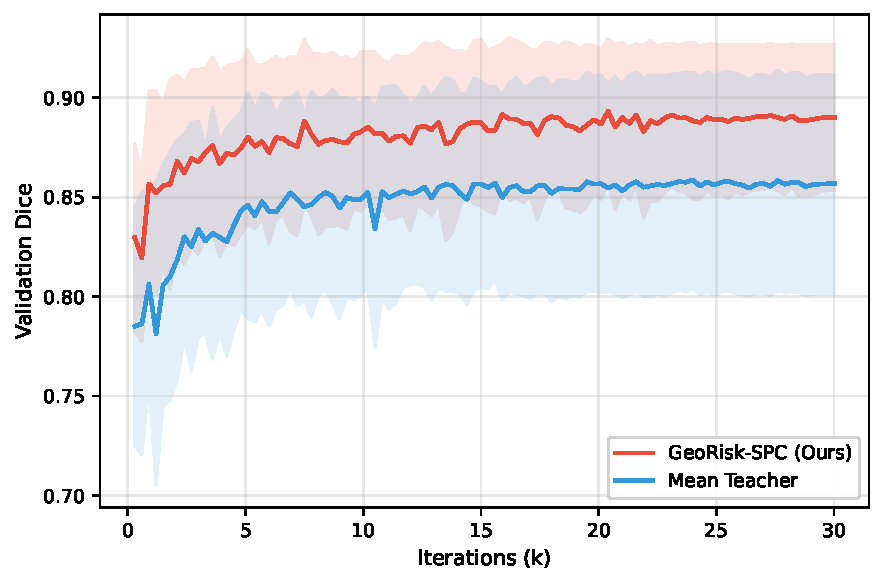
\includegraphics[width=\columnwidth]{figures/convergence.pdf}
\caption{Training curves of GeoRisk-SPC and Mean Teacher on EndoVis 2017 (20\% labeled data). GeoRisk-SPC converges faster and achieves higher final Dice score.}
\label{fig:convergence}
\end{figure}

\begin{figure}[t]
\centering
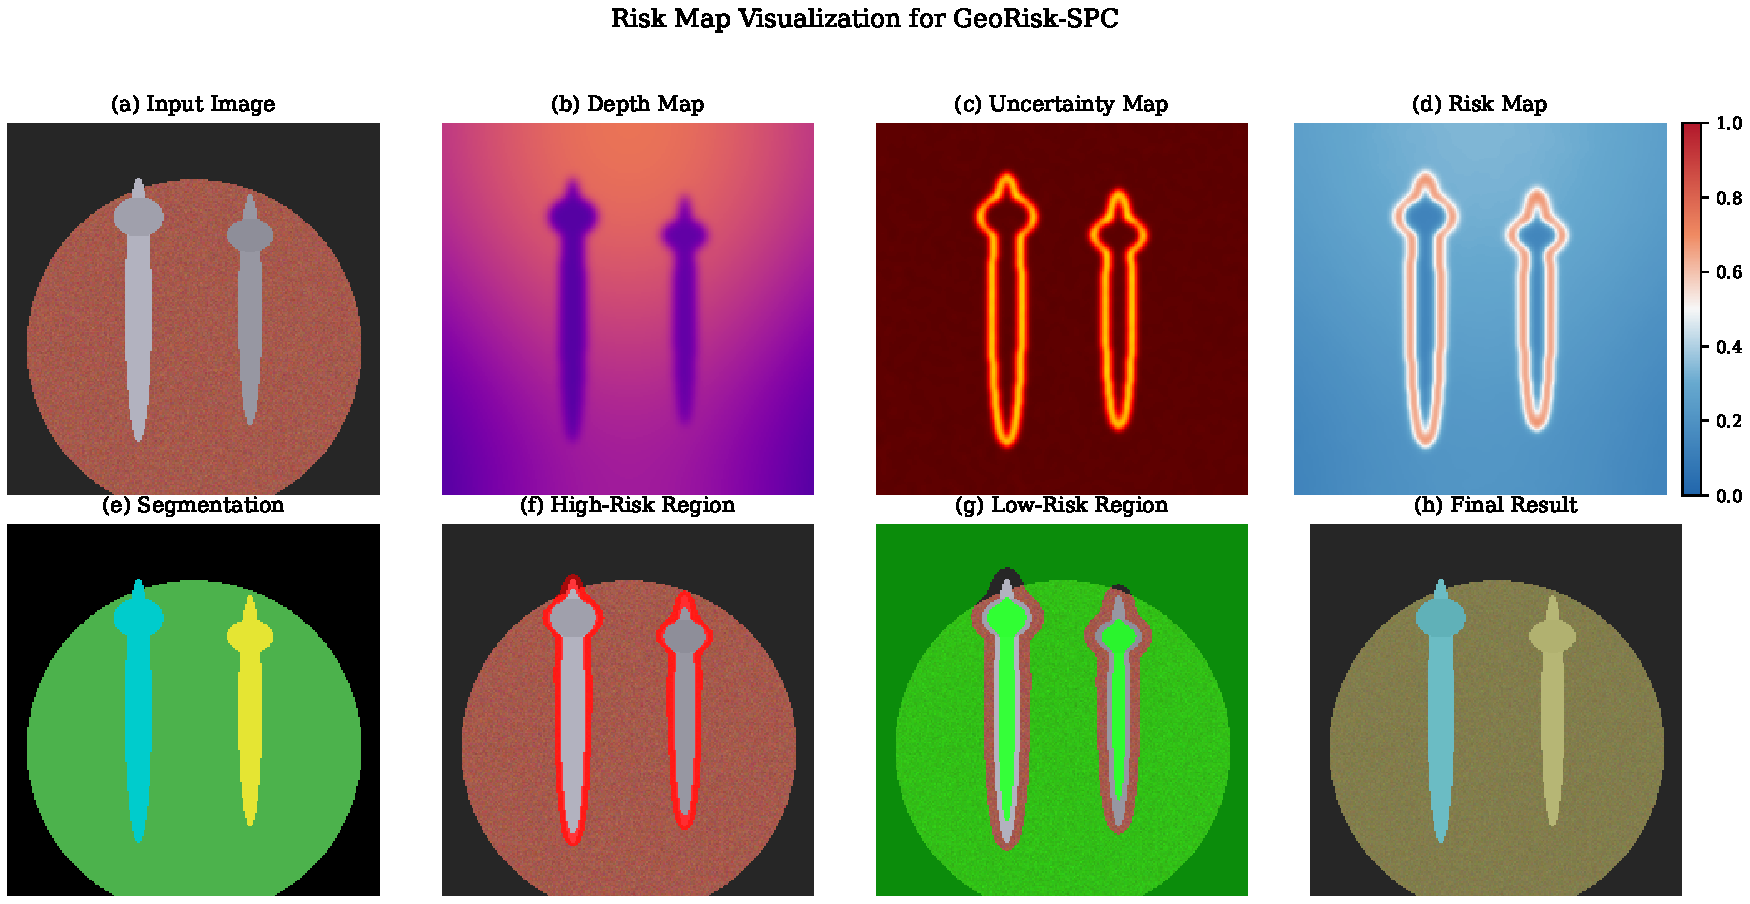
\includegraphics[width=\columnwidth]{figures/risk_map.pdf}
\caption{Visualization of risk maps. From left to right: input image, depth map, risk map, and segmentation result. High-risk regions (red) correspond to instrument boundaries and ambiguous areas.}
\label{fig:risk_map}
\end{figure}

\section{Discussion}

\subsection{Why Depth Discontinuity Works}
The effectiveness of depth discontinuity for risk localization stems from the physical properties of surgical scenes. Instrument boundaries typically correspond to depth changes due to the 3D structure of instruments and tissue. These depth discontinuities create ambiguity in pseudo-labels because:
\begin{itemize}
\item Small errors in depth estimation are amplified at boundaries
\item Texture variations near boundaries confuse the segmentation model
\item Motion blur during surgery is more pronounced at instrument edges
\end{itemize}
By explicitly identifying these regions, our method can apply appropriate supervision strategies rather than relying on potentially noisy pseudo-labels.

\subsection{Computational Overhead}
GeoRisk-SPC introduces minimal computational overhead. The risk localization module adds approximately 5\% to the training time compared to standard Mean Teacher. The dual-decoder architecture increases memory usage by about 30\%, but this is offset by the improved convergence speed (fewer iterations needed to reach optimal performance).

\subsection{Limitations}
Our method has several limitations:
\begin{itemize}
\item \textbf{Depth quality dependency}: The effectiveness of risk localization depends on the quality of pre-computed depth maps. Poor depth estimation may lead to inaccurate risk maps.
\item \textbf{Threshold sensitivity}: The performance is sensitive to the risk threshold $\tau_r$ and confidence threshold $\tau_c$. Adaptive thresholding strategies could be explored in future work.
\item \textbf{Dataset specificity}: We only evaluated on EndoVis 2017. Validation on more diverse surgical datasets is needed to confirm generalizability.
\end{itemize}

\section{Conclusion}
We proposed GeoRisk-SPC for semi-supervised surgical instrument segmentation. By leveraging depth discontinuity as geometric prior, our method effectively identifies high-risk regions in pseudo-labels and applies targeted consistency learning. The region-aware supervision strategy combines hard pseudo-labels for reliable regions with soft consistency constraints for ambiguous regions. Structural perturbation consistency further improves robustness by performing risk-guided feature perturbation.

Our key insight is that depth discontinuity from monocular depth estimation correlates with instrument boundaries, providing valuable geometric priors for identifying unreliable pseudo-label regions. This observation enables us to design a principled framework that differentiates between reliable and unreliable regions, applying appropriate supervision strategies to each.

Experiments on EndoVis 2017 demonstrate that GeoRisk-SPC achieves 92.15\% Dice with 20\% labeled data, 91.15\% Dice with 40\% labeled data, 88.59\% Dice with 10\% labeled data, and 86.68\% Dice with only 5\% labeled data, consistently outperforming existing methods including MT, UAMT, and URPC across all settings. The improvement is particularly significant in low-label regimes, demonstrating the effectiveness of our approach when annotation resources are limited.

Future work includes extending our method to 3D surgical scene segmentation and exploring additional geometric priors such as surface normals and instrument pose estimation. We also plan to investigate adaptive thresholding strategies for risk map generation to further improve the robustness of our approach.

\section*{Acknowledgment}
This work was supported by ...

\bibliographystyle{IEEEtran}
\bibliography{references}

\end{document}
